\documentclass[10pt, a4paper]{article} % 设置字体大小和纸张类型
\usepackage{ctex}
\usepackage{amsmath, amsfonts, amssymb} % 数学公式支持
\usepackage{graphicx} % 插入图片
\usepackage{hyperref} % 超链接支持
\usepackage{geometry}
\geometry{a4paper, margin=1.5cm} % 设置页边距

\title{电子电路基础第一次课外作业}
\author{吕俊霆 2024270901009}
\date{\today}

\begin{document}

\maketitle

\section{T1}
\subsection{题面}

\begin{figure}[htbp] % 图片浮动环境
    \centering
    \begin{minipage}[t]{0.48\textwidth} % 图片宽度占页面宽度的 48%
        \centering
        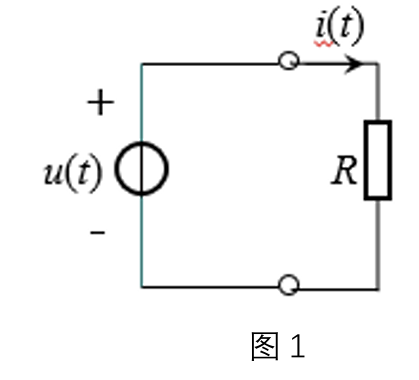
\includegraphics[width=\linewidth]{image/T1.png} % 图片宽度设置为 minipage 的宽度
        \label{fig:side:a}
    \end{minipage}
    \hfill % 添加一些水平间距
    \begin{minipage}[t]{0.48\textwidth} % 文本宽度占页面宽度的 48%
        图1所示电阻电路中,已知:$u\left(t\right) =  \sqrt{2}U\sin\omega t  $;$i\left(t\right)=\sqrt{2}I\sin\omega t$求电阻消耗的瞬时功
率p(t)(画出示意图)和平均功率P。
    \end{minipage}
\end{figure}
\subsection{解答}
$$
p(t) = u(t)\bullet i(t) = 2UI\sin^{2}\omega t
$$
\begin{figure}
    \centering
    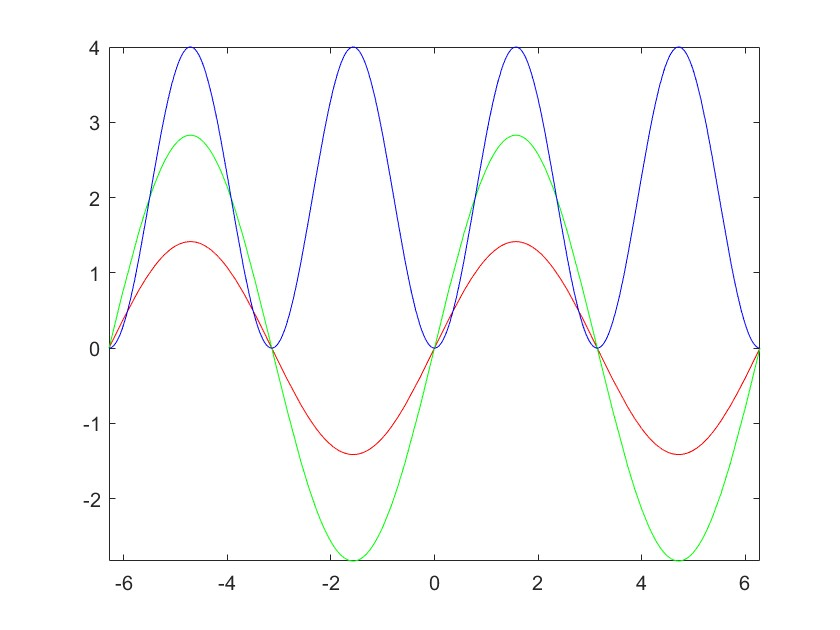
\includegraphics[width=0.3\textwidth]{image/T1.jpg}
    \caption{u(t)红,i(t)绿,p(t)蓝}
\end{figure}
据此可知平均功率为$\overline{p} = \sqrt{2}UI $

\clearpage

\section{T2}
\subsection{题面}
\begin{figure}[htbp] % 图片浮动环境
    \centering
    \begin{minipage}[t]{0.40\textwidth} % 图片宽度占页面宽度的 48%
        \centering
        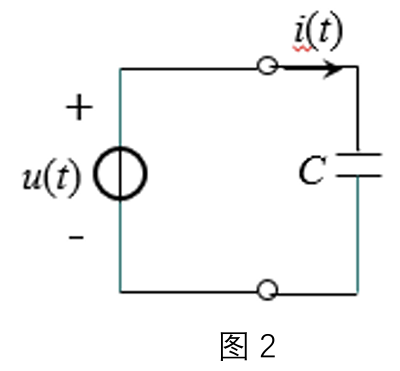
\includegraphics[width=\linewidth]{image/T2.png} % 图片宽度设置为 minipage 的宽度
        \label{fig:side:b}
    \end{minipage}
    \hfill % 添加一些水平间距
    \begin{minipage}[t]{0.66\textwidth} % 文本宽度占页面宽度的 48%


        图1所示电容电路中,已知:$u\left(t\right) =  \sqrt{2}U(\sin\omega t - 90°) $;$i\left(t\right)=\sqrt{2}I\sin\omega t $(因为电容的阻抗为$Z_{C}=\frac{1}{j\omega C}$,表明电容电压滞后电流90°)。求电容消耗的瞬时功率p(t)(画出示意图)和平均功率P。

    \end{minipage}
\end{figure}
\subsection{解答}
$$
p(t) = u(t)\bullet i(t) = -UI\sin2\omega t
$$
\begin{figure}[h]
    \centering
    \begin{minipage}[t]{\textwidth}
        \centering
        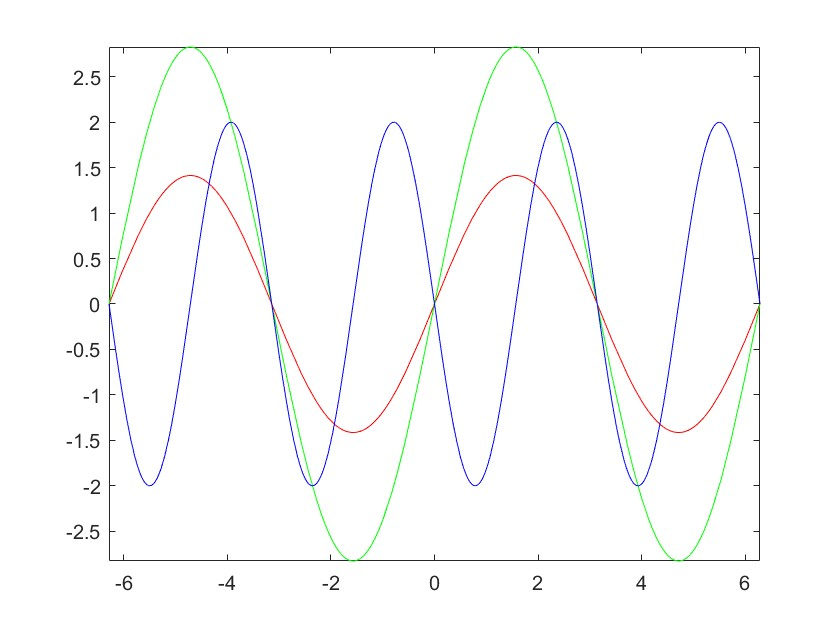
\includegraphics[width=0.3\textwidth]{image/T2.jpg}
    \caption{u(t)红,i(t)绿,p(t)蓝}
    \end{minipage}
    
\end{figure}
据此可知平均功率为$\overline{p} = 0 $

\clearpage

\section{T3}
\subsection{题面}
\begin{figure}[htbp] % 图片浮动环境
    \centering
    \begin{minipage}[t]{0.40\textwidth} % 图片宽度占页面宽度的 48%
        \centering
        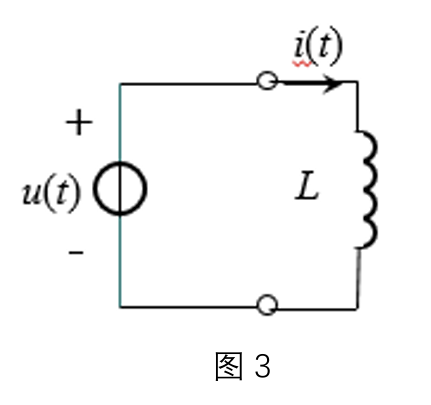
\includegraphics[width=\linewidth]{image/T3.png} % 图片宽度设置为 minipage 的宽度
        \label{fig:side:c}
    \end{minipage}
    \hfill % 添加一些水平间距
    \begin{minipage}[t]{0.66\textwidth} % 文本宽度占页面宽度的 48%


        图1所示电感电路中,已知:$u\left(t\right) =  \sqrt{2}U(\sin\omega t + 90°) $;$i\left(t\right)=\sqrt{2}I\sin\omega t $(因为电容的阻抗为$Z_{L}=j\omega L$,表明电感电压超前电流90°)。求电感消耗的瞬时功率p(t)(画出示意图)和平均功率P。

    \end{minipage}
\end{figure}

\subsection{解答}
$$
p(t) = u(t)\bullet i(t) = UI\sin2\omega t
$$
\begin{figure}[ht]
    \centering
    \begin{minipage}[t]{\textwidth}
        \centering
        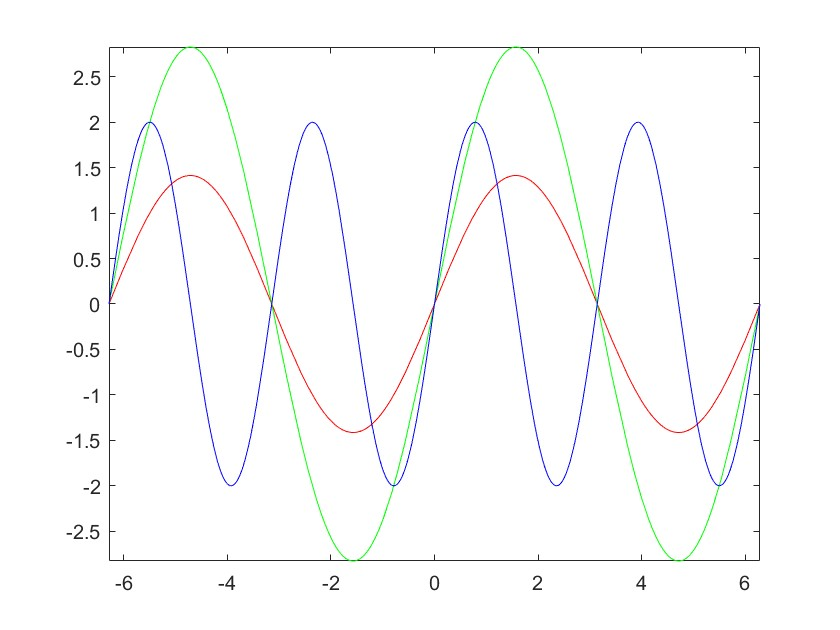
\includegraphics[width=0.3\textwidth]{image/T3.jpg}
    \caption{u(t)红,i(t)绿,p(t)蓝}
    \end{minipage}
    
\end{figure}
据此可知平均功率为$\overline{p} = 0 $

\clearpage

\section{T4}
\subsection{题面}
\begin{figure}[htbp] % 图片浮动环境
    \centering
    \begin{minipage}[t]{0.40\textwidth} % 图片宽度占页面宽度的 48%
        \centering
        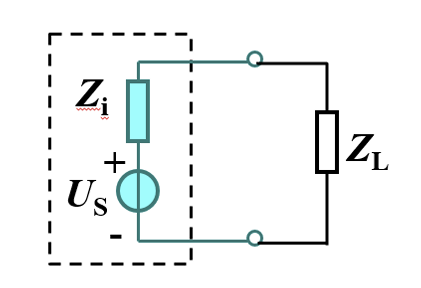
\includegraphics[width=\linewidth]{image/T4.png} % 图片宽度设置为 minipage 的宽度
        \caption{}
        \label{fig:side:d}
    \end{minipage}
    \hfill % 添加一些水平间距
    \begin{minipage}[t]{0.66\textwidth} 
        电路如图4所示,设$Z_{i} = R_{i} + jX_{i}, Z_{L} = R_{L} + jX_{L},$负载$Z_{L}$获得最大功率条件是$Z_{L} = Z_{i}^{*},$即$R_{L} = R_{i}, X_{L} = -X_{i}$(共轭匹配), 试证明?

    \end{minipage}
\end{figure}


\subsection{解答}
电路中, 负载阻抗$Z_{L} = R_{L}+jX_{L}$, 内阻抗$Z_{i} = R_{i} + jX_{i}$。通过负载的电流为 $I = \frac{U_{s}}{Z_{i} + Z_{L}}$, 负载的功率\(P_{L}\)为$P_{L} = I^2\cdot R_{L} = \left\lvert I\right\rvert^2\cdot R_{L} = \left\lvert \frac{U_{S}}{Z_{i} + Z_{L}}\right\rvert^2 \cdot R_{L}  $

化简得到$$P_{L} = \frac{U_{S}^2\times R_{L}}{\left\lvert Z_{i} + Z_{L}\right\rvert^2 }$$可知需要让分母最小, 将分母进行展开得到$$\left\lvert Z_{i} + Z_{L}\right\rvert^2 = \left\lvert R_{i} + jX_{i} + R_{L} + jX_{L}\right\rvert^2 = (R_{i}+R_{L})^2 + (X_{i} + X_{L})^2 $$

经计算可得, 当$R_{L} = R_{i}$且$X_{L} = -X_{i}$, 即$Z_{L} = Z_{i}^*$时,$\left\lvert Z_{i} + Z_{L}\right\rvert^2 $取最小值, 使得负载$Z_{L}$获得最大功率

\end{document}
